\documentclass{beamer}
\usepackage{beamerthemeshadow}
\usepackage{graphicx}
\usepackage{color}
\usepackage[utf8]{inputenc}
\usepackage{hyperref}
\usepackage[flushleft]{threeparttable}
\definecolor{UBCblue}{rgb}{0.04706, 0.13725, 0.26667} % UBC Blue (primary)
\definecolor{UBCgrey}{rgb}{0.3686, 0.5255, 0.6235} % UBC Grey (secondary)

\setbeamercolor{palette primary}{bg=UBCblue,fg=white}
\setbeamercolor{palette secondary}{bg=UBCblue,fg=white}
\setbeamercolor{palette tertiary}{bg=UBCblue,fg=white}
\setbeamercolor{palette quaternary}{bg=UBCblue,fg=white}
\setbeamercolor{structure}{fg=UBCblue} % itemize, enumerate, etc
\setbeamercolor{section in toc}{fg=UBCblue} % TOC sections

% Override palette coloring with secondary
\setbeamercolor{subsection in head/foot}{bg=UBCgrey,fg=white}
\usepackage[T1]{fontenc}
\usepackage[english,serbian]{babel}


\def\d{{\fontencoding{T1}\selectfont\dj}}
\def\D{{\fontencoding{T1}\selectfont\DJ}}


\title{Tehničko i naučno pisanje}
\subtitle{-- Svemir kao velika neuronska mreža --}
\author{Aleksa Filipović, Marta Kiso, Veljko Seničanin, \\Luka Stamenković}
\institute{Matematički fakultet\\Univerzitet u Beogradu}
\date{
	\footnotesize{Beograd, 2022.}	
}

\begin{document}
\begin{frame}
	\thispagestyle{empty}
	\titlepage
\end{frame}

\addtocounter{framenumber}{-1}

\begin{frame}[fragile]\frametitle{Literatura}
	\begin{itemize}
		\item Zasnovano na seminarskom radu:\\
        „Svemir kao velika neuronska mreža - Aleksa Filipović, Marta Kiso, Veljko Seničanin, Luka Stamenković”, koji se može naći na sledećem linku: (\url{https://github.com/LukaStamenkovic/20_TNP2022/blob/main/20_FilipovicKisoSenicaninStamenkovic.pdf/})
	\end{itemize}
\end{frame}

\begin{frame}
	\frametitle{Pregled} % Table of contents slide, comment this block out to remove it
	\tableofcontents[hidesubsections]
\end{frame}

\section{Uvod}

\begin{frame}[fragile]\frametitle{Uvod}
	\begin{itemize}	
        \item Začetnik ideje je ruski naučnik Vitali Vančurin (Vitaly Vanchurin)
		\item Bazirana na sličnosti svemira i ljudskog mozga
        \item Naučnici su zaključili da u mozgu ima oko 70 milijardi neurona, dok u svemiru postoji oko 100 milijardi galaksija
        \item Mreže čine samo po oko 30\% ukupne mase
        \end{itemize}
       \begin{figure}[h]
        \centering
        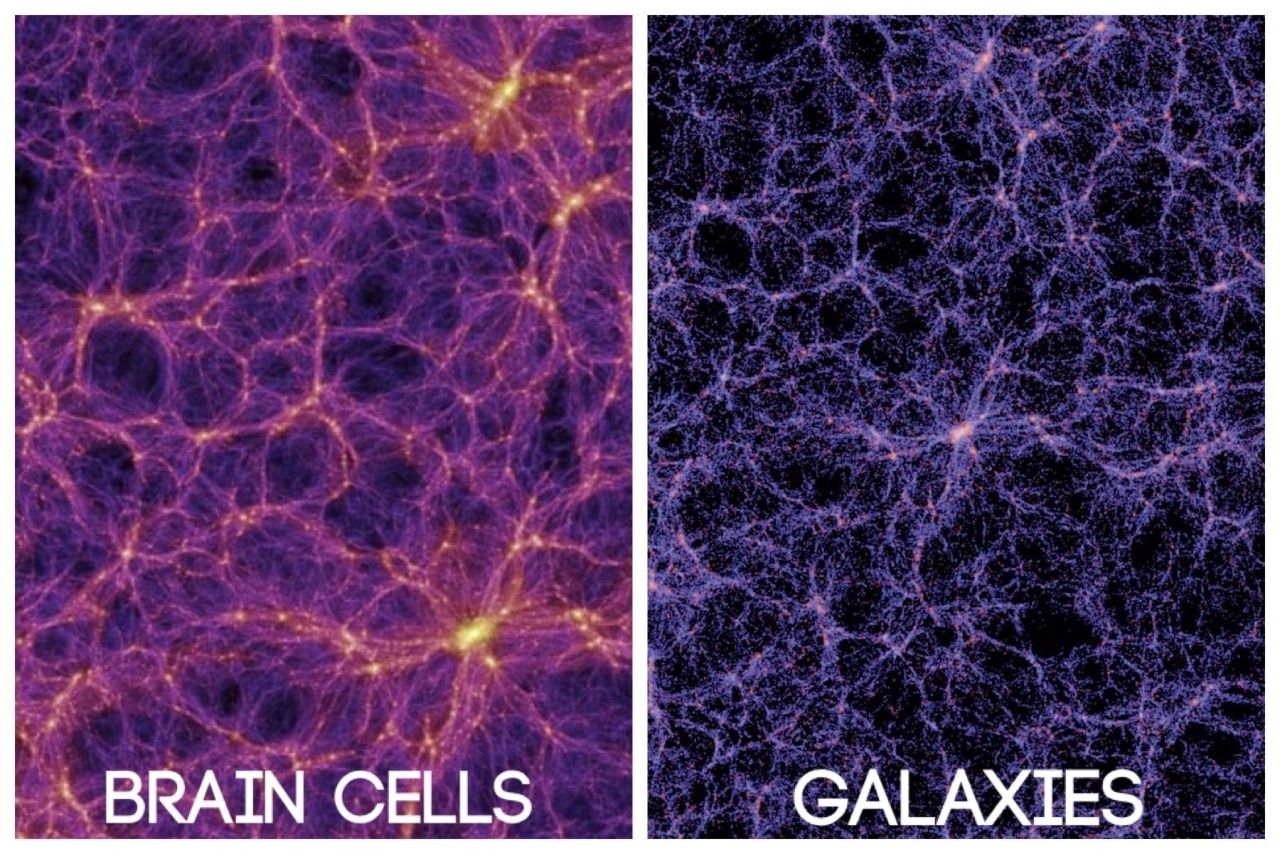
\includegraphics[width=50mm,height=30mm, scale=0.5]{komparacija.jpeg}
        \label{fig:komparacija.jpeg}
        \end{figure}
        \end{frame}
        
\subsection{Povezanost fizike i svemira}
\begin{frame}[fragile]\frametitle{Povezanost fizike i svemira}
\begin{itemize}	
        \item Ako posmatramo svemir kao neuronsku mrežu, možemo ga opisati zakonima kvantne fizike
        \item \textbf{Dinamika učenja neuronskih mreža je veoma slična kvantnoj dinamici}
        \item Moguća solucija neslaganja klasične i kvantne fizike
      \end{itemize} 

\begin{table}[h!]
\begin{center}
{\footnotesize
\begin{tabular}{|c|c|c|} \hline
 & Klasična fizika& Kvantna fizika\\ \hline
Svojstva& čestična ili talasna & i čestična i talasna\\ \hline
Pozicija i brzina& mogu se tačno odrediti& ne mogu se  tačno odrediti\\ \hline 
Dilatacija vremena& ne postoji & postoji \\ \hline
Kontrakcija dužine& ne postoji& postoji\\ \hline
\end{tabular}
\caption{Razlike između klasične i kvantne fizike}
\label{tab:tabela1}
}
\end{center}
\end{table}

 
\end{frame}



\section{Neuronske mreže}
    \begin{frame}[fragile]\frametitle{Neuronske mreže}
	   \begin{itemize}	
            \item Neuronske mreže predstavljaju najpopularniju i jednu od najprimenjenijih metoda mašinskog učenja
            \item Neke od primena su
            \begin{itemize}
                \item Medicinska dijagnostika
                \item Prepoznavanje objekata na slikama
                \item Autonomna vožnja
            \end{itemize}
		  \item Vrste neuronskih mreža
            \begin{itemize}
                \item Potpuno povezane neuronske mreže
                \item Konvolutivne neuronske mreže
                \item Rekurentne neuronske mreže
                \item Grafovske neuronske mreže
            \end{itemize}
	   \end{itemize}
    \end{frame}

\section{Vančurijev rad}
    \begin{frame}[fragile]\frametitle{Vančurijev rad}
        \begin{itemize}
            \item Pokušao da spoji kvantnu mehaniku i teoriju relativiteta
            \item Svet oko nas je velika neuronska mreža
            \item Pokušaji obrazloženja i problem posmatrača
            \item Mikroskopska neuronska struktura kao osnov svega
            \item Stav o paralelnim unverzumima
        \end{itemize}
    \end{frame}

\section{Istraživanja}
    \begin{frame}[fragile]\frametitle{Istraživanja}
	   \begin{itemize}	
            \item Pored Vančurija i mnogi drugi naučnici su se bavili pitanjem svemira kao velike neuronske mreže
            \item Kristof Koh, ljudski mozak nazvao 'najsloženijim objektom u poznatom svemiru'
	   \end{itemize}
   
          \begin{figure}[h]
           \centering
           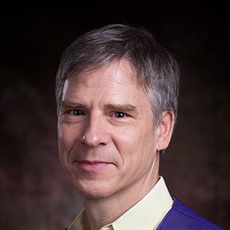
\includegraphics[width=35mm,height=30mm, scale=0.5] 
             {koh.jpg}
          \label{fig:koh.jpg}
          \end{figure}
          \end{frame}
          
\subsection{Franko Vaza i Alberto Feleti}
    \begin{frame}[fragile]\frametitle{Franko Vaza i Alberto Feleti}
	   \begin{itemize}	
		  \item Franko Vaza i Alberto Feleti su opisali sličnosti između neuronske i galaktičke mreže
            \begin{itemize}
                \item Svemir ima približan broj galaksija, koliko naš mozak ima ćelija 
                \item kompjuterska simulacija kosmičke mreže i presek moždanog tkiva imaju sličnu strukturu
                \item obe mreže imaju sličan spektar snage i stepen kompleksnosti 
                \item autori su zaključili da su obe strukture, strukture koje se same organizuju
            \end{itemize}
	   \end{itemize}
    \end{frame}

 \subsection{Donald Hofman i Dmitri Krijukov}
    \begin{frame}[fragile]\frametitle{Donald Hofman i Dmitri Krijukov}
	   \begin{itemize}	
		  \item Donald Hofman smatra da prirodna selekcija je favorizovala percepciju koja skriva istinu i vodi nas prema korisnim radnjama
		  \item Dmitri Krijukov je jedan od glavnih autora studije koja pokazuje da svemir raste na isti način kao mozak
	   \end{itemize}
          \begin{figure}[h]
           \centering
           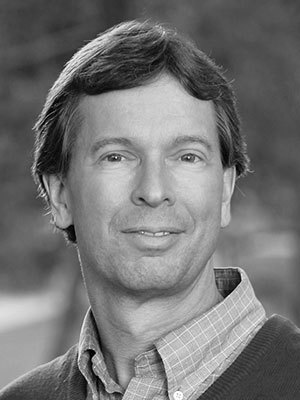
\includegraphics[width=27mm,height=30mm, scale=0.5] 
             {hoffman.jpg}
          \label{fig:hoffman.jpg}
          \end{figure}
    \end{frame}


\section{Diskusija}
    \begin{frame}[fragile]\frametitle{Diskusija}
	   \begin{itemize}	
            \item Glavni novi uvid je da kvantna mehanika možda nije fundamentalna teorija, već samo matematički alat koji omogućava izvo\dj enje statističkih proračuna u odre\dj enim dinamičkim sistemima.
		  \item Ako je to tačno, onda bi trebalo da se izvedu svi bitni elementi (kompleksna talasna funkcija, Šredingerova jednačina, itd.) iz prvog principa.
		  \item U svom radu Vančurin radi upravo to za dinamički sistem neuronske mreže. Ovo pokazuje da neuronske mreže zaista mogu opisati kvantne pojave ali takođe i klasične pojave.
	   \end{itemize}
    \end{frame}


\section{Zaključak}
    \begin{frame}[fragile]\frametitle{Zaključak}
	   \begin{itemize}	
            \item  U ovom radu smo razmatrali mogućnost da je ceo univerzum na svom najosnovnijem nivou neuronska mreža. To bi se moglo smatrati predlogom teorije svega
            \item  Sve što je potrebno je pronaći jedan fizički fenomen koji se ne može opisati neuronskim mrežama. Nažalost (ili na sreću), lakše je to reći nego učiniti
		  \item  Neuronske mreže nude zanimljivu novu perspektivu
	   \end{itemize}
    \end{frame}

\end{document}